% ----------------------------------------------------------
\chapter{Comportamento Mecânico de Túneis}
% ----------------------------------------------------------

\section{Influência da escavação e o conceito de convergência da seção}

De uma forma geral, do ponto de vista do maciço, a escavação de um túnel nada mais é do que uma perturbação no seu estado natural de equilíbrio devido à remoção de parte do maciço. Essa perturbação induzirá o maciço a uma nova configuração de equilíbrio que mobilizará tensões tangenciais desviando, dessa forma, a direção das tensões principais no entorno da escavação. Através desse \textbf{arqueamento das tensões}, o próprio maciço participa da sustentação da cavidade. Esse arqueamento pode ser decomposto em dois arcos longitudinais (contidos nos planos horizontal e vertical) e um arco transversal (no plano perpendicular ao eixo do túnel), tal como mostrado na \autoref{arqueamento}.

\begin{figure}[H]
	\begin{center}
		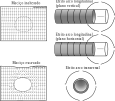
\includegraphics[scale = 1]{0401-efeito_arco.pdf}
	\end{center}
	\caption{\label{arqueamento}Ilustração do arqueamento das tensões principais (adaptado de: \citeonline[p. 10-11]{Franca2006})}
\end{figure}

A presença dos três arcos na zona que acompanha a frente de escavação faz com que essa região tenha um campo de deslocamentos tridimensional convergente em direção à face de escavação. No entanto, conforme essa frente avança e se afasta, apenas o arqueamento transversal se mantém, fazendo com que o campo de deslocamentos seja bidimensional contido no plano transversal ao eixo do túnel. Em vista disso, é conveniente caracterizar três zonas no interior do maciço: uma zona não perturbada pela escavação, uma zona de influência da frente de escavação e uma zona livre dessa influência (\autoref{campo_frente_escavacao}).

\begin{figure}[H]
	\begin{center}
		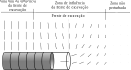
\includegraphics[scale = 1]{0402-campo vetorial de deslocamentos no maciço.pdf}
	\end{center}
	\caption{\label{campo_frente_escavacao}Campo vetorial de deslocamentos no maciço durante a escavação de um túnel (adaptado de: \citeonline[p. 12]{Franca2006})}
\end{figure}

O parâmetro geométrico mais simples e representativo do comportamento de um túnel é o fechamento de sua cavidade, também conhecido como \textbf{convergência}. Se um túnel circular estiver em um maciço homogêneo, isotrópico, submetido a um estado de tensões inicial geostático hidrostático, o campo de deslocamentos no entorno de uma seção fora da zona de influência da frente de escavação estará contido no plano transversal e será puramente radial, podendo ser expresso por uma função  $u(r)$. Nesse caso, a convergência $U$ é definida pela razão entre o deslocamento da cavidade e seu raio inicial $U=-u(r=R)/R$. A presença do sinal negativo é opcional e serve para que a convergência fique positiva se a seção diminuir, ou seja, $u(R) < 0$  (\autoref{definicao_convergencia}).

\begin{figure}[H]
	\begin{center}
		
\includegraphics[scale = 1]{0403-convergencia de uma seção circular.pdf}
	\end{center}
	\caption{\label{definicao_convergencia}Ilustração das medidas geométricas que compõe a convergência de uma seção circular: a) corte transversal, b) corte longitudinal}
\end{figure}

Dependendo da anisotropia das tensões \textit{in situ} ou do formato da seção, sua deformada pode não ser radial e, na prática, podem-se usar varias medidas para compor o cálculo da convergência da seção (\autoref{convergenca_secao_qualquer}).

\begin{figure}[H]
	\begin{center}
		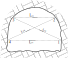
\includegraphics[scale = 1]{0404-convergencia de uma seção qualquer.pdf}
	\end{center}
	\caption{\label{convergenca_secao_qualquer}Medição da convergência em quatro direções de uma seção não circular (adaptado de: \citeonline[p. 8]{Panet1995})}
\end{figure}

Outro aspecto importante para determinar a influência da escavação e caracterizar o comportamento global do túnel é a representação gráfica das convergências ao longo do seu eixo longitudinal, conhecida como \textbf{perfil de convergências}. Por exemplo, com o objetivo de quantificar a extensão da zona de influência da frente da escavação, Hanafy \& Emery (1980) graficaram o perfil de convergências do seu modelo de um túnel circular em um maciço homogêneo, isotrópico e elástico linear (Figura 4.5).

\section{Mecanismos de ruptura em túneis profundos}

\section{Influência da reologia do maciço}

\subsection{Comportamento instantâneo}

\subsection{Comportamento diferido no tempo}

\subsection{Alguns estudos considerando leis elastoplásticas e viscoplásticas}

\section{Influência da forma da seção}

\section{Influência da profundidade do túnel}

\section{Influência da proximidade da superfície}

\section{Influência do revestimento e parâmetros adimensionais}

\section{Método convergência-confinamento}




